\pagebreak
\subsection{Rysunki}
    \vspace{20px}
    \begin{figure}[ht]
        \centering
        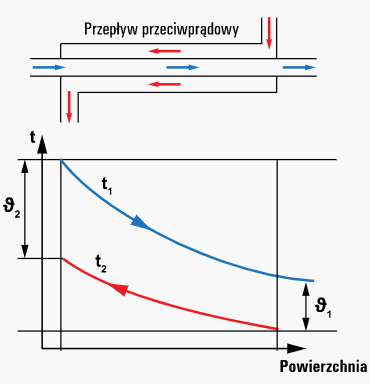
\includegraphics[width=\linewidth-250px]{Przeciwprąd.png}
            \caption{Uproszczony shemat wymiennika ``Rura w rurze`` w układzie przepływu przeciwprądowego oraz wykres przedstawiający temperaturę czynników dla takiego układu.}
        \centering
        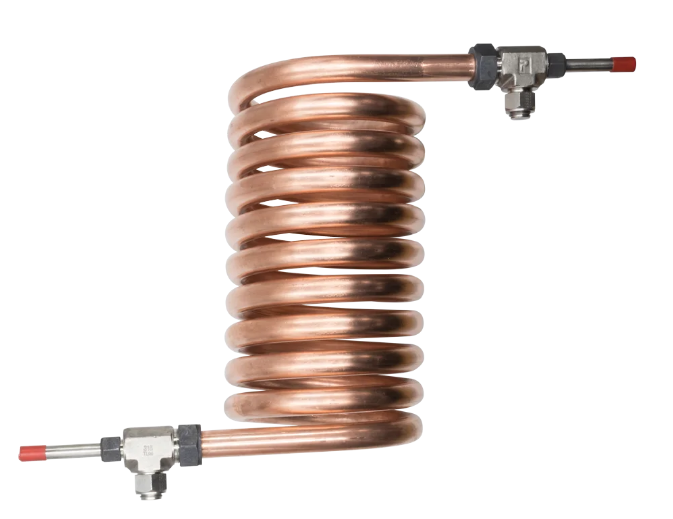
\includegraphics[width=\linewidth-250px]{Wymiennik.PNG}
            \caption{Poglądowy rysunek wymiennika typu ``Rura w rurze - rury gięte``. }
    \end{figure}

